\newcounter{num}
\setcounter{num}{1} % !!!!!!!!! 1-English CV; 2 - Chinese CV !!!!!!!!!!!

\documentclass[10pt]{ctexart}
\usepackage[margin=0.8in]{geometry}
\usepackage{multirow,url,tabularx,booktabs}
\usepackage{fontspec}
\fontspec{Times New Roman} 

\usepackage{fancyhdr} 
\renewcommand{\headrulewidth}{0pt}
\usepackage{datetime} \yyyymmdddate
\usepackage{lastpage}
\pagestyle{fancyplain}
\fancyhf{}
\lfoot{ \fancyplain{}{\footnotesize \today} }
\rfoot{ \fancyplain{}{\footnotesize Page \thepage\ /\ \pageref{LastPage}} }

\usepackage[T1]{fontenc}
\usepackage[utf8]{inputenc}
\usepackage{mathptmx}

\usepackage{tikz}
\usetikzlibrary{calc}

% Spacing
\usepackage{setspace,enumitem}
\setlength{\parindent}{0em}
\setlist[itemize,1]{leftmargin=\dimexpr 1em}
\def\changemargin#1#2{\list{}{\rightmargin#2\leftmargin#1}\item[]}
\let\endchangemargin=\endlist 

\hyphenpenalty=5000
\tolerance=1000

% Multiple biagraphies
\usepackage[resetlabels]{multibib}
\newcites{Working}{Working}
\newcites{SCI}{SCI}
\newcites{EIJA}{EI Journal}
\newcites{EICA}{EI Conference}
\newcites{ChineseCore}{Chinese}
\newcites{Other}{other}

\usepackage{etoolbox}
\patchcmd{\thebibliography}{\section*{\refname}}{}{}{}

\usepackage{xpatch}
\makeatletter
\newcommand\removebibheader
  {\xpatchcmd\std@thebibliography
    {\section*{\refname}%
     \@mkboth{\MakeUppercase\refname}{\MakeUppercase\refname}%
    }{}{}{}%
  }
\makeatother

% table align and width
\usepackage{array}
\newcolumntype{L}[1]{>{\raggedright\let\newline\\\arraybackslash\hspace{0pt}}m{#1}}
\newcolumntype{C}[1]{>{\centering\let\newline\\\arraybackslash\hspace{0pt}}m{#1}}
\newcolumntype{R}[1]{>{\raggedleft\let\newline\\\arraybackslash\hspace{0pt}}m{#1}}

% section color
\usepackage{xcolor,lipsum}
\usepackage{titlesec}
\titleformat{name=\section}[block]
  {\large\raggedleft}
  {}
  {0pt}
  {\colorsection}
\titlespacing*{\section}{0pt}{\baselineskip}{\baselineskip}

\newcommand{\colorsection}[1]{%
  \colorbox{gray!15}{\parbox{\dimexpr\textwidth-2\fboxsep}{#1}}}

%%%%%%%%%%%%%%%%%%%%%%%%%%%%%%%%%%

\begin{document}
    \ifnum\value{num}<2 {
    \begin{table}[htbp]
    \begin{tabular}{R{0.2\linewidth}L{0.55\linewidth}L{0.18\linewidth}}
    \multicolumn{2}{c}{\huge{\textbf{\ifnum\value{num}<2 {Zhengru Ren}  \else{任 政 儒}\fi}}} & \multirow{7}[0]{*}{\vspace*{10em} 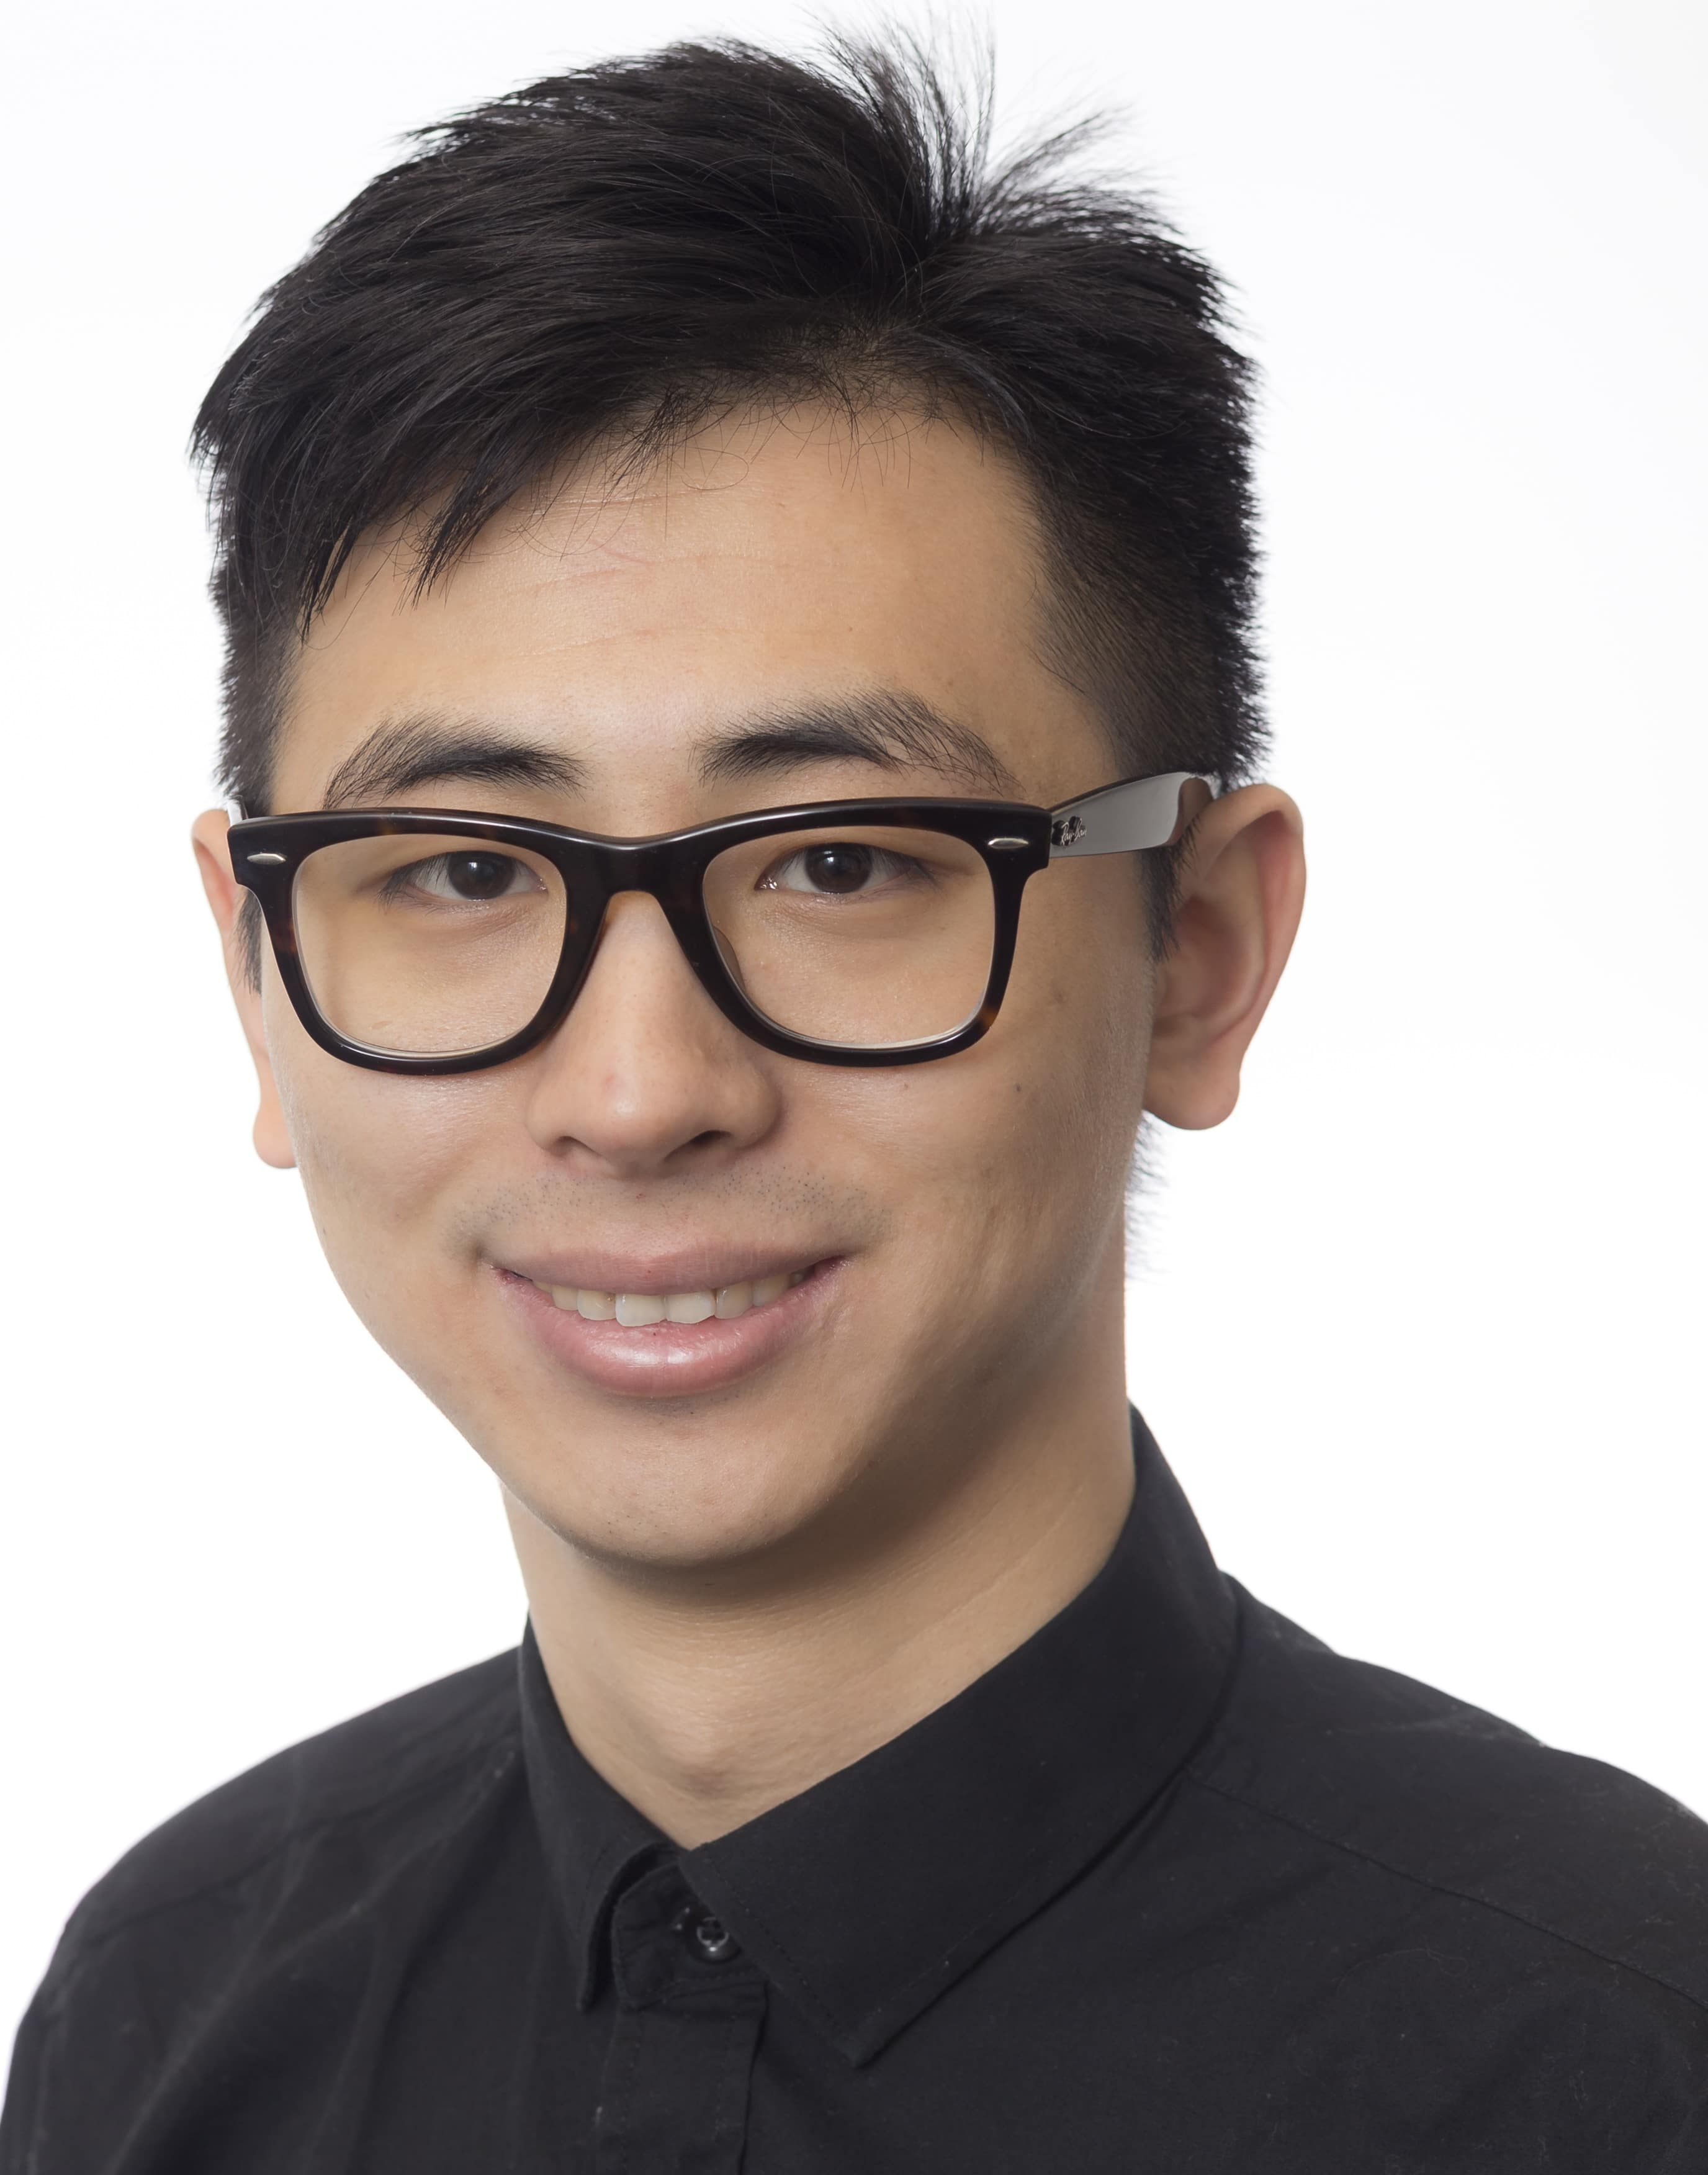
\includegraphics[width=0.7\linewidth]{images/photo-min.jpg}} \\
    \\
    % Date of birth: & 1989.10.19 &  \\
    Email: & zhengru.ren@ntnu.no, renzhengru@gmail.com &  \\
    Mobile: & +47~474~42~832 &  \\
    URL:  & https://www.zhengru.ren &  \\
    ORCID: & 0000-0001-5522-8094 \\
    Address:   & O. Nielsens Veg 10, Tyholt, N-7491 Trondheim, Norway &  \\
            \end{tabular}%
\end{table}%
}
    \else{
    \begin{table}[htbp]
    \begin{tabular}{R{0.2\linewidth}L{0.55\linewidth}L{0.18\linewidth}}
    \multicolumn{2}{c}{\huge{\textbf{\ifnum\value{num}<2 {Zhengru Ren}  \else{任政儒}\fi}}} & \multirow{7}[0]{*}{\vspace*{10em} 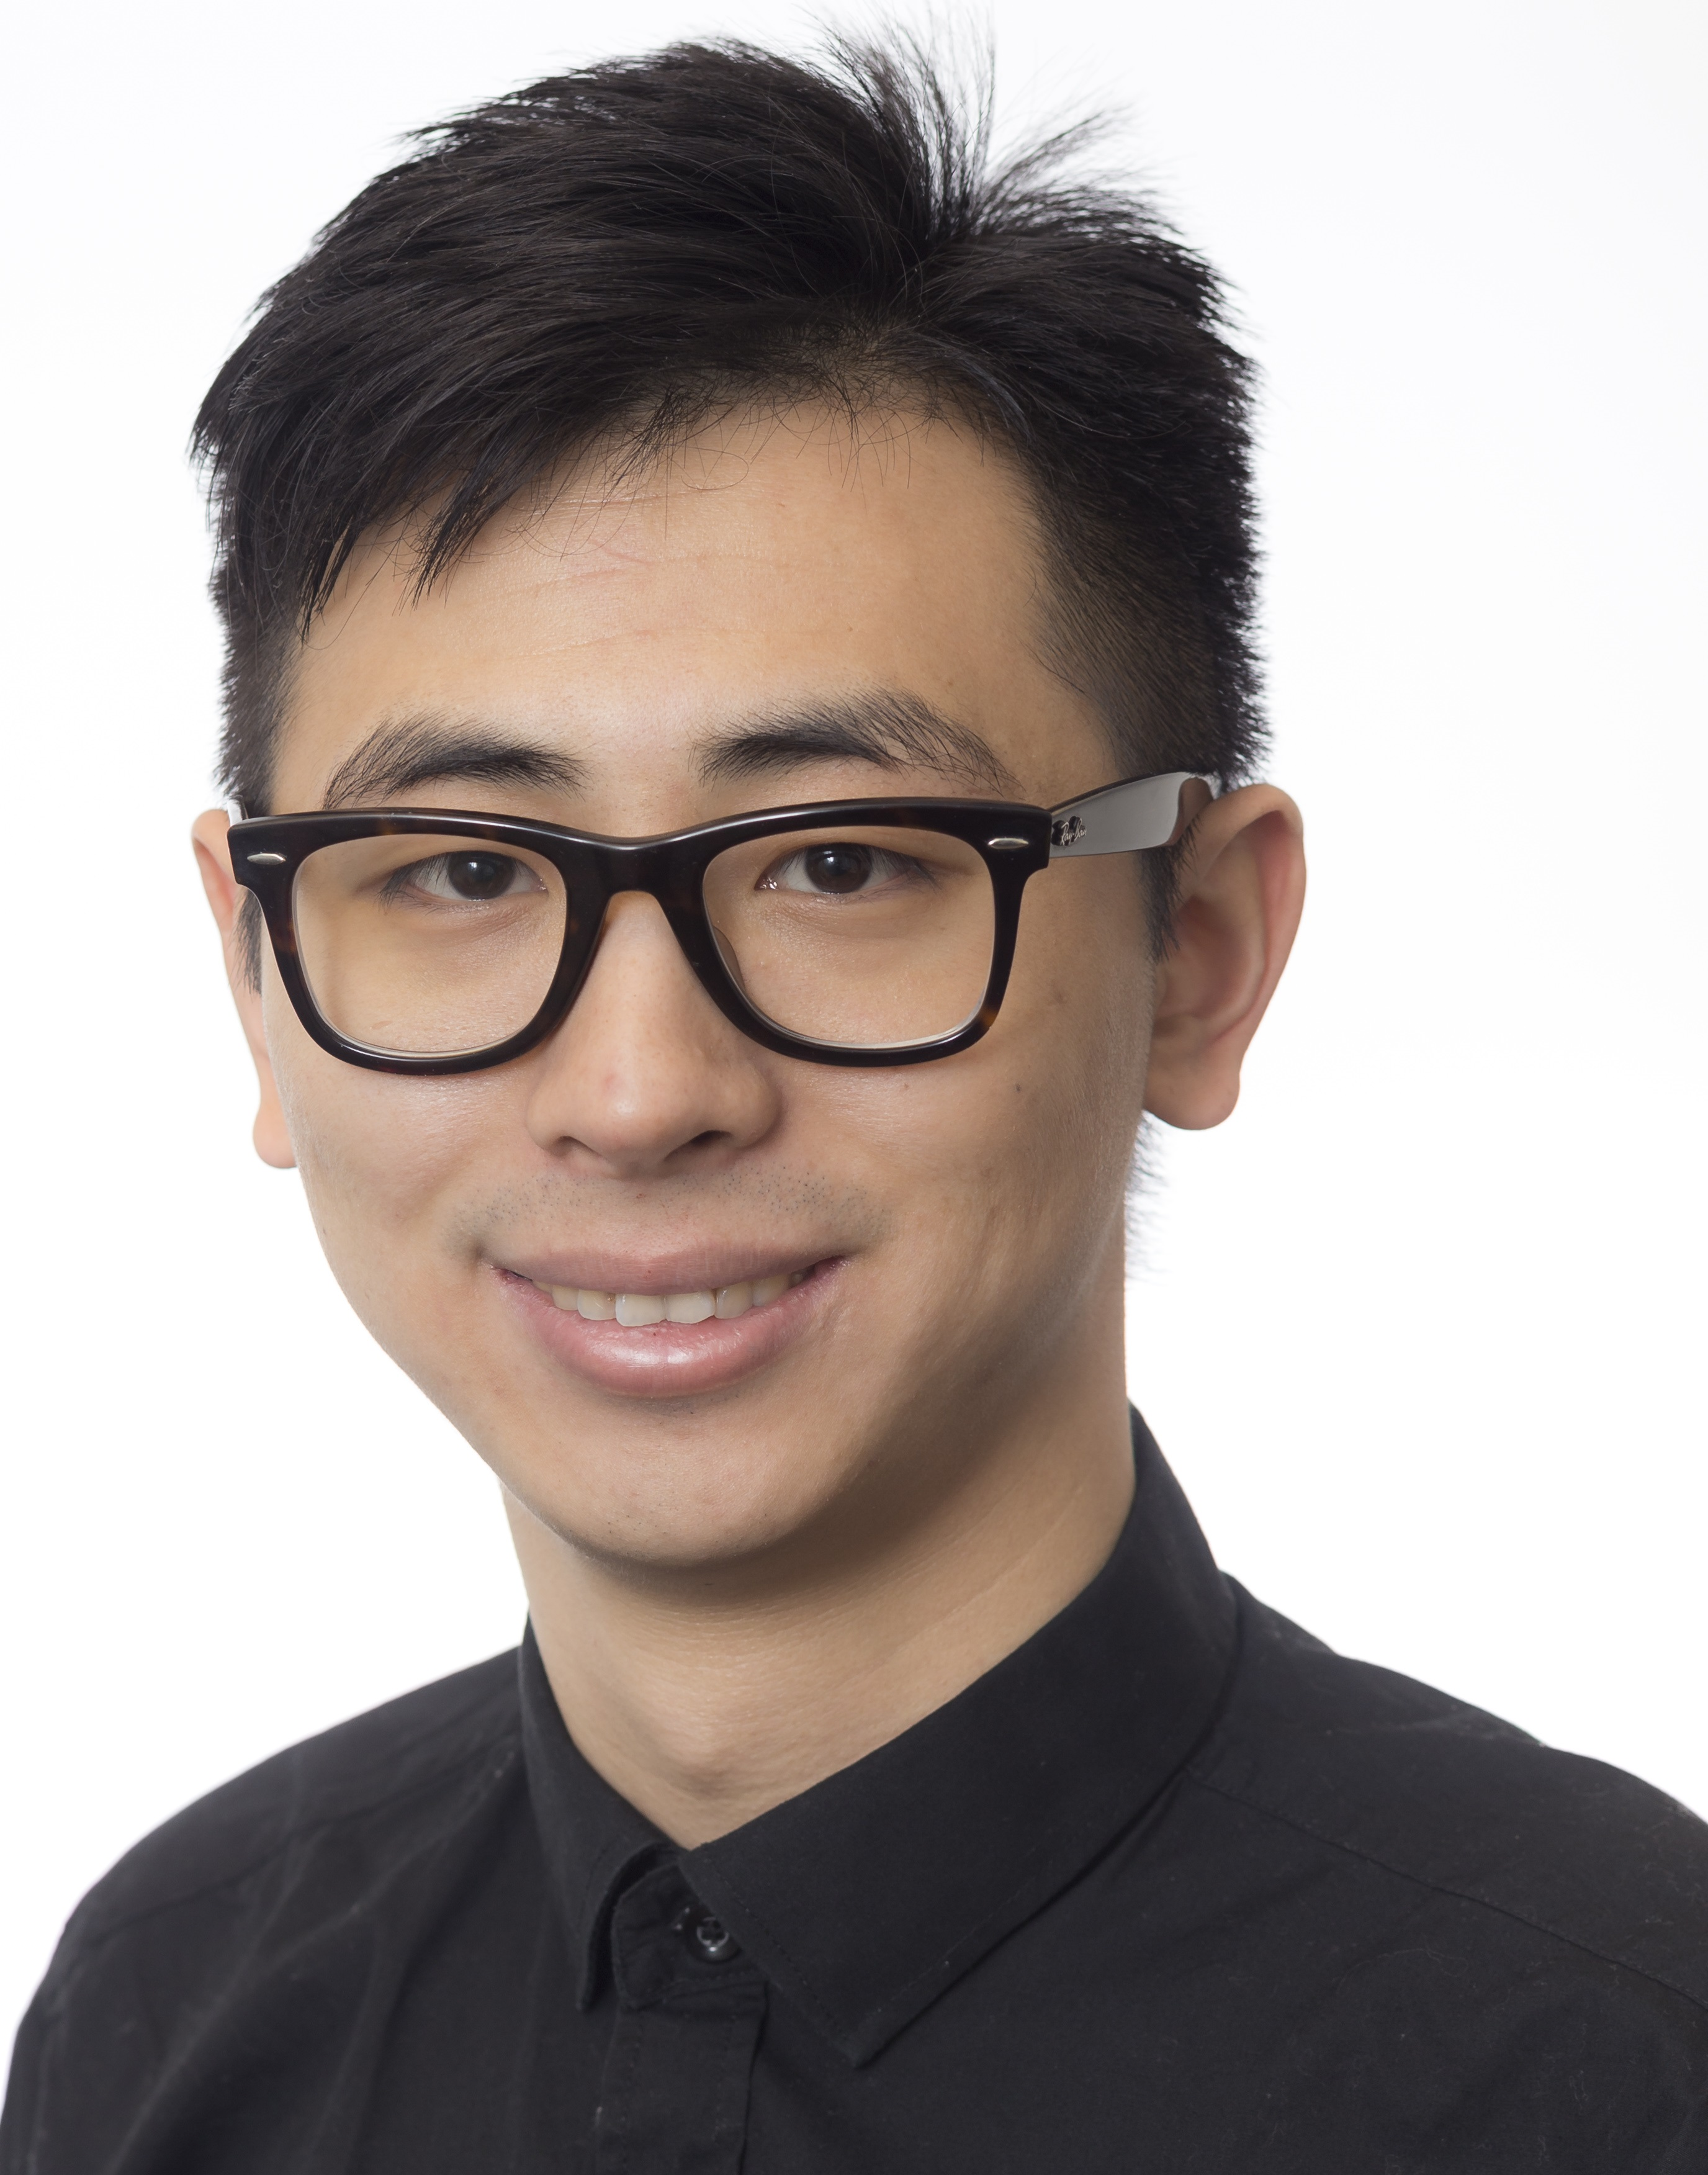
\includegraphics[width=0.7\linewidth]{images/photo.jpg}} \\
    \\
    出生日期: & 1989年10月19日 &  \\
    电子邮箱: & zhengru.ren@ntnu.no, renzhengru@gmail.com &  \\
    联系方式: & +47~474~42~832 &  \\
    个人主页:  & https://www.ntnu.edu/employees/zhengrur &  \\
    地址:   & O. Nielsens Veg 10, Tyholt, N-7491 Trondheim, Norway &  \\
        \end{tabular}%
\end{table}%
}\fi


\section*{\textbf{\ifnum\value{num}<2 {Work experience}  \else{工作经历}\fi}}
    \ifnum\value{num}<2 {
    \begin{tabular}{R{0.15\columnwidth}L{0.63\columnwidth}L{0.17\columnwidth}}
    2019.8 -- Present & \textbf{Postdoctoral researcher}, Department of Marine Technology  & Trondheim, Norway \\
    & Norwegian University of Science and Technology (NTNU) & \\
          & \multicolumn{2}{l}{Centre for Research-based Innovation of Marine Operations (SFI MOVE)} \\
          & \multicolumn{2}{l}{- Topic: Onboard decision support system} \\
    2016.4 -- 2019.8 & \textbf{Researcher}, Department of Oceans Operations and Civil Engineering  & {\AA}lesund, Norway \\
    & \multicolumn{2}{l}{Norwegian University of Science and Technology}\\
    & \multicolumn{2}{l}{- Topic: Simulation and control of floating wind turbine installation}
    \end{tabular}%
    }
    \else{
    \begin{table}[htbp]
    \begin{tabular}{R{0.15\columnwidth}L{0.55\columnwidth}L{0.3\columnwidth}}
    2019.8 -- 至今 & 博士后研究员,海洋技术学院,挪威科技大学 & 特隆赫姆, 挪威 \\
          & \multicolumn{2}{l}{Centre for Research-based Innovation of Marine Operations (SFI MOVE)} \\
          & \multicolumn{2}{l}{- 课题: 智能舰载决策支持系统(基于船体运动的波浪谱估计及船体模型修正)} \\
    2019.4 -- 2019.8 & 研究员, 海洋操作与土木工程学院, 挪威科技大学 & 奥勒松, 挪威 \\
    & \multicolumn{2}{l}{- 课题: 浮式风机一体化安装数值模拟与自动控制}
    \end{tabular}%
\end{table}%
    }
    \fi
\vspace*{0.5em}

\section*{\textbf{\ifnum\value{num}<2 {Education}  \else{教育背景}\fi}}
\ifnum\value{num}<2 {
    \begin{tabular}[t]{R{0.15\columnwidth}L{0.63\columnwidth}L{0.17\columnwidth}}
    2016.1 -- 2019.8 & \textbf{Ph.D.}, Department of Marine Technology & Trondheim, Norway \\
    	& \multicolumn{2}{l}{Norwegian University of Science and Technology}\\
          & \multicolumn{2}{l}{Centre for Research-based Innovation of Marine Operations (SFI MOVE)} \\
          & \multicolumn{2}{l}{Centre for Autonomous Marine Operations and Systems (NTNU AMOS)} \\
          & \multicolumn{2}{l}{- Thesis: Advanced control algorithms to support automated offshore wind turbine installation} \\
          & \multicolumn{2}{l}{- Main supervisor: Roger Skjetne, Co-supervisor: Zhen Gao} \\
          &       &  \\
    2013.8 -- 2015.6 & \textbf{MSc.} in Marine Technology (Specialization in Marine Cybernetics) & Trondheim, Norway \\
    & \multicolumn{2}{l}{Norwegian University of Science and Technology}\\
          & \multicolumn{2}{l}{- Thesis: Fault-tolerant control of thruster-assisted position mooring system} \\
          & \multicolumn{2}{l}{- Supervisor: Roger Skjetne} \\
          &       &  \\
    2008.9 -- 2012.6 & \textbf{B.Eng.} in Ocean Engineering, Dalian University of Technology & Dalian, China \\
          & \multicolumn{2}{l}{- Thesis: The schematic design of a 19000DWT production oil tanker} \\
    \end{tabular}%
}\else{
\begin{table}[htbp]
    \begin{tabular}{R{0.15\columnwidth}L{0.55\columnwidth}L{0.3\columnwidth}}
    2016.1 -- 2019.8 & 学位: 博士,挪威科技大学 & 特隆赫姆, 挪威 \\
          & \multicolumn{2}{l}{Centre for Research-based Innovation of Marine Operations (SFI MOVE)} \\
          & \multicolumn{2}{l}{Centre for Autonomous Marine Operations and Systems (NTNU AMOS)} \\
          & \multicolumn{2}{l}{专业: 海洋技术} \\
          & \multicolumn{2}{l}{- 论文题目: 海上固定式及浮式风机的自动安装及决策支持系统} \\
          & \multicolumn{2}{l}{- 主导师: Roger Skjetne, 副导师: Zhen Gao} \\
          &       &  \\
    2013.8 -- 2015.6 & 学位: 硕士,挪威科技大学, & 特隆赫姆, 挪威 \\
          & \multicolumn{2}{l}{专业: 海洋技术(海洋控制学方向)} \\
          & \multicolumn{2}{l}{- 论文题目: 推进器辅助系泊定位系统的容错控制} \\
          & \multicolumn{2}{l}{- 导师: Roger Skjetne} \\
          &       &  \\
    2008.9 -- 2012.6 & 学位: 工学学士,大连理工大学 & 大连, 中国 \\
          & \multicolumn{2}{l}{ 专业: 船舶与海洋工程} \\
          & \multicolumn{2}{l}{- 论文题目: 19000DWT 成品油轮设计} \\
    \end{tabular}%
\end{table}%
}\fi
\vspace*{0.5em}

\section*{\textbf{\ifnum\value{num}<2 {Research interests}  \else{科研兴趣}\fi}}
\ifnum\value{num}<2 {
% \begin{changemargin}{2em}{0em} 
% \setlength{\baselineskip}{100.5 em}
Nonlinear control theory; sensor fusion; marine operation; offshore installation; sea state estimation; offshore wind turbine; renewable energy;  dynamic positioning (DP) system; thruster-assisted position mooring (TAPM) system; underwater robots;  fault diagnosis; multi-agent system; model tuning; digitalization.
% \end{changemargin}
% \item Machine learning, artificial intelligence 
}\else{
\begin{changemargin}{2em}{0em} 
\setlength{\baselineskip}{1.5 em}
% Nonlinear control theory; sensor fusion; marine operation; offshore installation; sea state estimation; offshore wind turbine; renewable energy;  dynamic positioning (DP) system; thruster-assisted position mooring (TAPM) system; underwater robots;  fault diagnosis; multi-agent system; model tuning; digitalization. 
非线性控制理论、传感器融合、海上作业、海上安装、海况估计、海上风机、海洋新能源、动力定位系统、动力辅助锚泊系统、水下机器人、容错控制、多智体控制、系统辨识、数字化孪生、强化学习
\end{changemargin}
}\fi
\vspace*{0.5em}

\section*{\textbf{\ifnum\value{num}<2 {Teaching experience}  \else{教学经历}\fi}}
\ifnum\value{num}<2 {
    \begin{minipage}{\textwidth}
    \textbf{MR8500 - PhD Topics in Marine Control Systems, NTNU, 2020}
    \begin{itemize}[label={}] \setlength\itemsep{0.5em}
    \item Lectures: Backstepping design on complex nonlinear systems.
    \end{itemize}
    \end{minipage}
}\else{
    \begin{minipage}{\textwidth}
    \textbf{MR8500 - PhD Topics in Marine Control Systems, 挪威科技大学, 2020}
    \begin{itemize}[label={}] \setlength\itemsep{0.5em}
    \item 课程: Backstepping design on complex nonlinear systems.
    \end{itemize}
    \end{minipage}
}\fi
\vspace*{0.5em}

\section*{\textbf{\ifnum\value{num}<2 {Supervision experience}  \else{指导学生}\fi}}
\begin{minipage}{\textwidth}
\textbf{\ifnum\value{num}<2 {Co-supervision of PhD student at NTNU}  \else{担任副导师指导博士生}\fi}
\begin{itemize}[label={}] \setlength\itemsep{0.5em}
    \item Behfar Ataei, 2019.8--2022.6, Virtual prototyping of installation of offshore power systems.
\end{itemize}
\end{minipage}
\vspace*{0.5em}

\textbf{\ifnum\value{num}<2 {Co-supervision of master students at NTNU}  \else{担任副导师指导硕士生}\fi}
\begin{itemize}[label={}] \setlength\itemsep{0.5em}
    \item Sindre Sagsveen Sl{\aa}ttum, 2020.8--2021.6, Load and sea state estimation based on distributed IMUs.
    \item Yuxuan Cai, 2020.8--2021.6, Data-driven condition monitoring of marine battery energy
    storage systems.
    \item Jens Nikolai Alfsen, 2019.8--2020.6, Dynamic optimal path-planning for autonomous harbor maneuvering.
    \item Caroline Sophie R{\o}hm Fleischer, 2019.8--2020.6, Optimal path-planning on a bio-inspired neural network landscape model for autonomous surface vessels.
    \item Hongyu Zhou, 2019.8--2020.6, Autonomous guidance, stepwise path planning, and path-following control with anti-collision for autonomous marine robots.
    \item Elias Gauslaa, 2019.8--2020.6, Navigation, guidance, and control for autonomous autodocking of ships.
    \item Jakob Stensvik Jensen, 2019.8--2020.6, Dynamic optimal path-planning for autonomous harbor maneuvering.
    \item Baiheng Wu, 2018.4--2019.1, Image processing and target tracking technology in the sea cucumber fishing application.
    \item Andreas Bro Kolst{\o}, 2017.9--2018.6, Fault detection for position mooring using statistical analysis.
    \item Ying Lu, 2017.9--2018.6, Current profile estimation for a moored floating structure.
\end{itemize}
\vspace*{0.5em}

\section*{\textbf{\ifnum\value{num}<2 {Academic experience}  \else{学术经历}\fi}}
\textbf{\ifnum\value{num}<2 {Participation research projects}  \else{主要科研项目}\fi}
\ifnum\value{num}<2 {
    \begin{itemize}[label={}] \setlength\itemsep{0.5em}
    \item \textbf{Norwegian Centre of Research-based Innovation SFI MOVE (Marine Operations in Virtual Environments)}\\
        \begin{tabular}[t]{R{0.15\columnwidth}L{0.8\columnwidth}}
        2016-2019 &  Project 5: Innovative installation of wind power systems\\
        2019-2021 &  Project 6: Onboard decision tool\\
        \end{tabular}%
    \item \textbf{Norwegian Centre of Excellence, NTNU AMOS (Centre for Autonomous Marine Operations and Systems)}
    \begin{tabular}[t]{R{0.15\columnwidth}L{0.8\columnwidth}}
        2016-2019 &  Project 3: Risk management and maximized operability of ships and ocean structures \\
    \end{tabular}%
    \item \textbf{Centre for Research-based Innovation SFI SAMCoT (Sustainable Arctic Marine and Coastal Technology)}\\
    \begin{tabular}[t]{R{0.15\columnwidth}L{0.8\columnwidth}}
        2019 &  Numerical simulations of moored floating structures in ice\\
    \end{tabular}%
    \end{itemize}
}\else{
    \begin{itemize}[label={}] \setlength\itemsep{0.5em}
    \item 2015 -- 2022 挪威研究创新中心计划,舰载决策支持系统,主要执行人
    \item 2015 -- 2022 挪威研究创新中心计划,海上风机安装,主要执行人
    \item 2017 -- 2020 上海交通大学海洋工程国家重点实验室开放课题, 海上风机新型安装技术研究, 第二完成人 %, 8万
    \item 2018 -- 2020 大连理工大学海岸和近海工程国家重点实验室开放课题, 被动式阻尼器对海上风机结构响应的影响, 第二完成人 %, 3万
    \end{itemize}
}\fi
\vspace*{0.5em}

\ifnum\value{num}<2 {
    \textbf{Funding/grants}
    \begin{itemize}[label={}] \setlength\itemsep{0.5em}
    \item Open Project of the State Key Laboratory of Ocean Engineering, Shanghai Jiao Tong University \\
    \begin{tabular}[t]{R{0.15\columnwidth}L{0.85\columnwidth}}
        2017 -- 2020 &  Research and development of innovative offshore wind farm installation techniques, second applicant\\
    \end{tabular}%
    \item Open Project of the State Key Laboratory of Coastal and Offshore Engineering, Dalian University of Technology\\
    \begin{tabular}[t]{R{0.15\columnwidth}L{0.85\columnwidth}}
        2018 -- 2020 &  The structural influence of passive damper to offshore wind turbine, second applicant\\
    \end{tabular}%
    \item Norwegian Ship Owner's Association's Fund, 2016, 2020
    \end{itemize}
    \vspace*{0.5em}
}\else{

}\fi

\section*{\textbf{\ifnum\value{num}<2 {Reviewer for international journals and conferences}  \else{国际期刊及会议审稿人}\fi}}
\begin{itemize}[label={}] \setlength\itemsep{0.5em}
\item Ocean Engineering%, 2019
\item Applied Ocean Research
\item Journal of Offshore Mechanics and Arctic Engineering%, 2018--2020
\item Journal of Marine Science and Engineering%, 2019
\item IEEE Transactions on Neural Networks and Learning Systems%, 2018
\item IEEE Transactions on Systems, Man, and Cybernetics: Systems
\item IEEE Access%, 2017--2019
\item Engineering Structures%, 2017--2020
\item Journal of Materials Research and Technology%, 2019--2020
\item International Journal of Energy Applications and Technologies%, 2018
\item Energies%, 2017--2019
%%%%%%%%%%%%%%%%%%%%%%%
\item IFAC Conference on Control Applications in Marine Systems (CAMS)%, 2016
\item International Conference on Ocean, Offshore and Arctic Engineering (OMAE)%, 2018--2020
\item International Offshore and Polar Engineering Conference (ISOPE)%, 2018
\item International Offshore Wind Technical Conference (IOWTC)%5, 2018
\item IFAC World Congress%, 2020
\end{itemize}
\vspace*{0.5em}

\section*{\textbf{\ifnum\value{num}<2 {Publications}  \else{科研成果}\fi}}
%%%%% Journals %%%%%
% 2021
\nociteSCI{ren:2021backsteppingReview,ren:20216DOFIdentification,ren:2021OWT_O&M_review,ren:2020complexShapedPayloadLifting,ren:2020seaStateEst,ren:2020preassemblyHydraulic,han:2020adaptive,han:2021ukf,amrit:2021LEE_energies,zhou:2020pathPlanning}
% 2020
\nociteSCI{ren:2020finiteTimeNNAdapticeCtrl,ren:2020IJOPE,verma:2020LEE_WE,verma:2020misalignment,verma:2020OMAE_resubmit,ming2019typeCTank,roger:2020TAPM_review}
% 2019
\nociteSCI{ren:2019bladeLift,ren:2019monopilePosition,verma:2019response,verma:2019impact,ming:2019iceOWT}
% 2018
\nociteSCI{ren:2018singleBladeInstallation,ren:2018highFidelityModel,xu:2018journalOMAE}
% 2017
\nociteSCI{jiang:2017parametric,jiang:2017review}
% Early
\nociteSCI{liang:2013generalized}

%%%%% Conference paper %%%%%
% 2020
\nociteEICA{verma:2020leadingEdge,zhiyu:2020damageIdentification}
% 2019
\nociteEICA{verma:2019OMAE}
% 2018
\nociteEICA{jin:2018installation,gao:2018probabilistic,ren:singleBladeInstallation3Lines,jiang:2018catamaranMating}
% 2017
\nociteEICA{ren:2017modeling,xu:2017}

\ifnum\value{num}<2 {
    % Early (\nociteEIJA)
    \nociteEIJA{ren:2016site,ren:2016tension,ren:2015tension,ren:2015supervisory}
    
    % Other conferences
    \nociteEICA{duan2019simcape,jin:2018installation,ni:2012software}
    
    %%%%% Chinese core %%%%%
    \nociteChineseCore{duan2019heaveCompensatorReview,ren:2014software}
 
    \textbf{SCI Journal papers}
    \bibliographystyleSCI{unsrt}{}
    \bibliographySCI{Quarterly_EN,bibtex_of_my_paper}  
    
    \textbf{EI Journal papers}
    \bibliographystyleEIJA{unsrt}
    \bibliographyEIJA{bibtex_of_my_paper}
    \vspace*{0.5em}
    
    \textbf{Chinese Core Journal papers}
    \bibliographystyleChineseCore{unsrt}
    \bibliographyChineseCore{bibtex_of_my_paper}
    \vspace*{0.5em}
    
    \vspace*{0.5em}
    \textbf{Conference papers}
    \bibliographystyleEICA{unsrt}
    \bibliographyEICA{bibtex_of_my_paper}
    \vspace*{0.5em}
    
   \textbf{CN Patents}
    \begin{enumerate}
    \item \textbf{任政儒}, 施伟, 宋兆波, 蒋致禹, 张礼贤, 由际昆. 实现双向合力控制的吊机延伸加装装置及双向张力控制吊车的方法, 2020.07.24, CN2019109320173 (发明专利)
    \item 施伟, 张礼贤, 蒋致禹, \textbf{任政儒}, 宁德志, 周利. 海上波能-风能集成系统及集成发电方法, 2020.06.02, CN2018116164404 (发明专利)
    \item 蒋致禹, \textbf{任政儒}, 施伟, 宁德志. 一种基于独立变桨的风电机组控制和制动方法, 2020.01.10, ZL2018108848638 (发明专利)
    \item \textbf{任政儒}, 蒋致禹, 施伟, 由际昆, 宁德志. 用于风机单叶片安装的主动反馈控制方法和装置, 2020.01.10, ZL2018108700240 (发明专利)
    \item \textbf{任政儒}, 蒋致禹, 施伟, 宁德志.基于锚链张力和立管上端角的水下流速剖面估计方法, 2019.12.17, CN2017110413343 (发明专利)
    \item \textbf{任政儒}, 蒋致禹, 施伟, 宁德志, 周利. 一种适用于水平轴风机的防叶片抛飞的安全装置, 2019.09.27, ZL2018100395983 (发明专利)
    \item \textbf{任政儒}, 蒋致禹, 施伟, 宁德志.一种锚泊海洋结构物锚链断裂的实时监测方法, 2019.06.21, ZL2017110426841 (发明专利)
    \end{enumerate}
    \vspace*{0.5em}
    
    \textbf{US Patents}
    \begin{enumerate}
    \item \textbf{任政儒}, 蒋致禹, 施伟, 宁德志. 一种用于海上风机塔筒安装的减摇装置, 申请日: 2017.9.11, 申请号: PCT/CN2017/101170, 美国专利申请号: US16340063, 进入主权国家日: 2019.04.09(美国专利)(已授权) 
    \item 蒋致禹, \textbf{任政儒}, 施伟, 宁德志. 一种适用于海上风机单叶片安装的轮毂对接装置, 申请日: 2017.9.11, 申请号: PCT/CN2017/101168, 美国专利申请号: US10837425B2, 进入主权国家日: 2019.04.05(美国专利)(已授权) 
    \item 施伟,蒋致禹,\textbf{任政儒},宁德志。一种新型浮式风能-波浪能联合发电系统,美国专利申请号:US16339570,公布日:2020.2.6公布号:US2020/0040865A1(美国专利)(已授权)
    \item 蒋致禹, \textbf{任政儒}, 施伟, 宁德志. 一种适用于海上单桩式风机安装的主动式阻尼装置, 申请日: 2018.2.28, PCT申请号PCT/CN2018/077522, 进入主权国家日: 2020.11.17(美国专利)(已授权) 
    \item 蒋致禹,任政儒,施伟,宁德志。一种适用于海上风机单叶片安装的轮毂对接装置,2020.11.17
    \end{enumerate}
    \vspace*{0.5em}
    
    \textbf{Patents under review}
    \begin{enumerate}
    \item 施伟, 周林, \textbf{任政儒}, 由际昆, 宁德志, 勾莹. 一种基于浮式风机和潮流能装置的深海能源集成系统, 申请日: 2018.03.06, CN Grant CN207960842U(实用新型), 申请号 201810211962X(发明专利) 
    \item 施伟, 蒋致禹, \textbf{任政儒}, 宁德志. 一种适用于近海的单桩式风能-波浪能集成发电系统, 申请日: 2017.11.09, CN, Grant CN207420785U (实用新型); 申请号: CN2017110985681 (发明专利)
    \item \textbf{任政儒}, 蒋致禹, 施伟, 宁德志.一种基于爆破的海上单桩风机的整体拆卸装置与方法, 申请日: 2018.01.08, CN, Grant CN207710215U (实用新型); 申请号: CN2018200263053 (发明专利)
    \item 蒋致禹, 施伟, 曾昕萌, \textbf{任政儒}, 张礼贤, 翟钢军. 适用于海上浮式风机安装的防波装置及其安装海上浮式风机的方法, 申请日: 2019.09.29, 申请号: CN2019109321335 
    \item \textbf{任政儒}, 蒋致禹, 施伟, 宁德志. 基于锚链张力的定位方法及卫星定位失灵的检测方法, 申请号: CN201711033438X
    \end{enumerate}
    \vspace*{0.5em}
    
}\else{
    % Early (\nociteEIJA)
    \nociteEIJA{ren:2016site,ren:2016tension,ren:2015tension,ren:2015supervisory}
    
    %%%%% Chinese core %%%%%
    \nociteChineseCore{zhou2021heaveCompensator,duan2019heaveCompensatorReview,ren:2014software}
    
    %%%%% Others %%%%%
    \nociteOther{duan2019simcape,jin:2018installation,ni:2012software} 
    
    \textbf{SCI期刊}
    \bibliographystyleSCI{unsrt}{}
    \bibliographySCI{Quarterly_CN,bibtex_of_my_paper}
    \vspace*{0.5em}
    
    \textbf{EI期刊}
    \bibliographystyleEIJA{unsrt}
    \bibliographyEIJA{bibtex_of_my_paper}
    \vspace*{0.5em}
    
    \textbf{EI会议}
    \bibliographystyleEICA{unsrt}
    \bibliographyEICA{bibtex_of_my_paper}
    \vspace*{0.5em}
    
    \textbf{中文核心}
    \bibliographystyleChineseCore{unsrt}
    \bibliographyChineseCore{bibtex_of_my_paper}
    \vspace*{0.5em}
    
    \textbf{其他}
    \bibliographystyleOther{unsrt}
    \bibliographyOther{bibtex_of_my_paper}
    \vspace*{0.5em}
    
    \textbf{国家发明专利}
    \begin{enumerate}
    \item \textbf{任政儒}, 施伟, 王亚坡, 张松浩, 宋兆波, 周波, 万岭. 一种适用于海上或陆上的负载载荷吊装主动减摇控制方法,2021.03.26, 申请号: CN2020100044236 (发明专利)
    \item 施伟, 张礼贤, 蒋致禹, \textbf{任政儒}, 宁德志, 周利. 海上波能-风能集成系统及集成发电方法,2020.03.17, ZL2018116164404 (发明专利)
    \item \textbf{任政儒}, 蒋致禹, 施伟, 由际昆, 宁德志. 用于风机单叶片安装的主动反馈控制方法和装置, 2020.01.10, ZL2018108700240 (发明专利)
    \item 蒋致禹, \textbf{任政儒}, 施伟, 宁德志. 一种基于独立变桨的风电机组控制和制动方法, 2020.01.10, ZL2018108848638 (发明专利)
    \item \textbf{任政儒}, 蒋致禹, 施伟, 宁德志.基于锚链张力和立管上端角的水下流速剖面估计方法, 2019.12.17, CN2017110413343 (发明专利)
    \item \textbf{任政儒}, 蒋致禹, 施伟, 宁德志, 周利. 一种适用于水平轴风机的防叶片抛飞的安全装置, 2019.09.27, ZL2018100395983 (发明专利)
    \item \textbf{任政儒}, 蒋致禹, 施伟, 宁德志.一种锚泊海洋结构物锚链断裂的实时监测方法, 2019.06.21, ZL2017110426841 (发明专利)
    \end{enumerate}
    \vspace*{0.5em}
    
    \textbf{国际发明专利}
    \begin{enumerate}
    \item \textbf{任政儒}, 蒋致禹, 施伟, 宁德志. 一种用于海上风机塔筒安装的减摇装置, 申请日: 2017.9.11, 申请号: PCT/CN2017/101170, 美国专利申请号: US16340063, 进入主权国家日: 2019.04.09(国际专利)(已授权) 
    \item 蒋致禹, \textbf{任政儒}, 施伟, 宁德志. 一种适用于海上风机单叶片安装的轮毂对接装置, 申请日: 2017.9.11, 申请号: PCT/CN2017/101168, 美国专利申请号: US10837425B2, 进入主权国家日: 2019.04.05(国际专利)(已授权) 
    \item 蒋致禹, \textbf{任政儒}, 施伟, 宁德志. 一种适用于海上单桩式风机安装的主动式阻尼装置, 申请日: 2018.2.28, PCT申请号PCT/CN2018/077522 , 
    蒋致禹,任政儒,施伟,宁德志。一种适用于海上风机单叶片安装的轮毂对接装置,2020.11.17
    \item 施伟, 蒋致禹, \textbf{任政儒}, 宁德志. 一种新型浮式风能-波浪能联合发电系统, 申请日: 2017.9.11, 申请号: PCT/CN2017/101165, 美国专利申请号: US16339570, 进入主权国家日: 2019.04.04(国际专利)(进入国家阶段)
    \end{enumerate}
    \vspace*{0.5em}
    
    \textbf{已授权实用新型专利, 发明专利待审批}
    \begin{enumerate}
    \item 施伟, 周林, \textbf{任政儒}, 由际昆, 宁德志, 勾莹. 一种基于浮式风机和潮流能装置的深海能源集成系统, 申请日: 2018.03.06, CN Grant CN207960842U(实用新型), 申请号 201810211962X(发明专利) 
    \item 施伟, 蒋致禹, \textbf{任政儒}, 宁德志. 一种适用于近海的单桩式风能-波浪能集成发电系统, 申请日: 2017.11.09, CN, Grant CN207420785U (实用新型); 申请号: CN2017110985681 (发明专利)
    \item \textbf{任政儒}, 蒋致禹, 施伟, 宁德志.一种基于爆破的海上单桩风机的整体拆卸装置与方法, 申请日: 2018.01.08, CN, Grant CN207710215U (实用新型); 申请号: CN2018200263053 (发明专利)
    \end{enumerate}
    \vspace*{0.5em}
    
    \textbf{发明公布}
    \begin{enumerate}
    \item \textbf{任政儒}, 施伟, 宋兆波, 蒋致禹, 张礼贤, 由际昆. 实现双向合力控制的吊机延伸加装装置及双向张力控制吊车的方法, 申请日: 2019.09.29, 申请号: CN2019109320173
    \item 蒋致禹, 施伟, 曾昕萌, \textbf{任政儒}, 张礼贤, 翟钢军. 适用于海上浮式风机安装的防波装置及其安装海上浮式风机的方法, 申请日: 2019.09.29, 申请号: CN2019109321335 
    \item \textbf{任政儒}, 蒋致禹, 施伟, 宁德志. 基于锚链张力的定位方法及卫星定位失灵的检测方法, 申请号: CN201711033438X
    \end{enumerate}
    \vspace*{0.5em}
}\fi

\section*{\textbf{\ifnum\value{num}<2 {Other experience}  \else{其他经历}\fi}}
\ifnum\value{num}<2 {
    \textbf{Fellowships and awards}
    \begin{itemize}[label={}] \setlength\itemsep{0.5em}
    \item PhD fellowship, SFI MOVE/NTNU AMOS, NTNU, 2016--2018
    \item Excellence prize, National Computer Program-Designing Competitions, China, 2012
    \item Outstanding graduates, DLUT, 2012
    \item 3rd prize, National Modern Distance Education and Practice Teaching High-End Academic BBS, China, 2011
    \item Provincial 2nd and 3rd prize, National 3D Innovation Design Competition, Liaoning, 2011
    \item National 1st prize, BeiDou-Cup China Adolescents Science \& Technology Innovation Contest, China, 2011
    % \item Social work scholarship, DLUT, 2009--2011
    % \item Cultural and sports activities scholarship, DLUT, 2010
    \end{itemize}
}\else{
    \textbf{奖学金及获奖情况}
    \begin{itemize}[label={}]
    \item 挪威科技大学全额博士奖学金, 2016--2018
    \item 全国大学生计算机程序设计大赛优秀奖, 2012
    \item 大连理工大学优秀毕业生, 2012
    \item 全国教育教学创新与发展高端论坛, 三等奖, 2011
    \item 辽宁省3D建模大赛省二等奖、省三等奖, 2011
    \item ``北斗杯''全国青少年科技创新大赛全国一等奖, 2011
    \item 大连理工大学社会实践奖学金, 2009--2011
    \item 大连理工大学文体活动奖学金, 2010
    \end{itemize}
}\fi
\vspace*{0.5em}

\ifnum\value{num}<2 {
    \textbf{Computer Skills}
    \begin{itemize}[label={}]
    \item MATLAB, Simulink, LabVIEW, 20-SIM, Maple, VB, C/C++, R, FORTRAN, Arduino
    \item ProE, UG, Inventor, Rhino, AutoCAD
    \item HAWC2, FAST, Fluent, Ansys, SIMA, DeepC, ShipX, Latex, PhotoShop
    \end{itemize}
    \vspace*{0.5em}
    
    \textbf{Language proficiency}
    \begin{itemize}[label={}] \setlength\itemsep{0.5em}
    \item Chinese: Native
    \item English: Fluent
    \item Norwegian: A2
    \end{itemize}
    \vspace*{0.5em}
}\else{

}\fi

\newpage
\ifnum\value{num}<2 {
    \section*{\textbf{Referees}}
    % \begin{table}[htbp]%
    % \begin{tabular*}{\linewidth}{@{\extracolsep\fill}ll@{\extracolsep\fill}}
    	\begin{tabular}{@{}l@{}}
    	\textbf{Roger Skjetne}\\
    	Professor of Marine Control Engineering\\
    	Department of Marine Technology\\
        Norwegian University of Science and Technology\\
        O. Nielsens Veg 10, Tyholt, N-7491 Trondheim, Norway \\
        \url{roger.skjetne@ntnu.no}, +47 92813672
        \end{tabular}\\
        \\ \\
        \begin{tabular}{@{}l@{}}
        \textbf{Zhen Gao}\\
        Professor of Marine Structures\\
    	Department of Marine Technology\\
        Norwegian University of Science and Technology\\
        O. Nielsens Veg 10, Tyholt, N-7491 Trondheim, Norway\\
        \url{zhen.gao@ntnu.no}, +47 91751114
        \end{tabular}\\
      \\ \\
        \begin{tabular}{@{}l@{}}
        \textbf{Karl Henning Halse}\\
        Associate Professor, Vice Dean for the bachelor education\\
    	Department of Ocean Operations and Civil Engineering\\
        Norwegian University of Science and Technology\\
        NTNU {\AA}lesund, Postboks 1517, NO-6025 {\AA}lesund, Norway\\
        \url{karl.h.halse@ntnu.no}, +47 95227613
        \end{tabular}\\
        \\ \\
        \begin{tabular}{@{}l@{}}
        \textbf{Zhiyu Jiang}\\
        Associate Professor\\
    	Department of Engineering Sciences\\
        Univerisity of Adger\\
        D3103, Jon Lilletuns vei 9, NO-4879, Grimstad, Norway\\
        \url{zhiyu.jiang@uia.no}, +47 37233489
        \end{tabular}
    % \end{tabular*}
    % \end{table}
}\else{

}\fi

\end{document}